\documentclass[11pt]{article}

\usepackage[utf8]{inputenc}
\usepackage[T1]{fontenc}
\usepackage[margin=1in]{geometry}
\usepackage{amsmath,amssymb,amsthm}
\usepackage{graphicx}
\usepackage{booktabs}
\usepackage{algorithm}
\usepackage{algpseudocode}
\usepackage{caption}
\usepackage{subcaption}
\usepackage{placeins}
\usepackage{xcolor}
\usepackage[colorlinks=true,linkcolor=black,citecolor=black,urlcolor=blue!55!black]{hyperref}

\newtheorem{proposition}{Proposition}
\newtheorem{definition}{Definition}
\newtheorem{remark}{Remark}

\newcommand{\R}{\mathbb{R}}
\newcommand{\rwL}{\mathcal{L}}
\newcommand{\Hop}{\mathbf{H}}
\newcommand{\norm}[1]{\left\lVert#1\right\rVert}
\newcommand{\conv}{\operatorname{conv}}

\title{\bf Heat-Kernel Context Compression:\\
Continuous-Time Diffusion for Token-Efficient\\ Language-Model Inference}

\author{Shashank Reddy Vadyala\\
\texttt{vadyala.shashankreddy@gmail.com}}

\date{\today}

\begin{document}
\maketitle

\begin{abstract}
\noindent
Most of what a large language model costs at inference time is tokens, and a great many of
those tokens are redundant. Retrieval and long-context prompts are the worst offenders: they
pack the prefill with near-duplicate text and pay full input rate for context the model never
really uses. We attack this with \emph{Heat-Kernel Context Compression} (HKCC). The idea is to
place the context tokens on a similarity graph and run the graph heat equation over their
embeddings. Heat flow erases high-frequency detail first, so how far a token drifts under
diffusion---its \emph{heat residual} $\rho_i(\tau)=\norm{x_i-[e^{-\tau\rwL}X]_i}$---measures how
much it stands apart from its neighbors. Distinctive tokens become anchors; the rest are folded
into diffused, multiplicity-weighted centroids. The merge is the part that matters: deleting
redundant tokens is ruinous, while re-expressing their mass costs almost nothing. A single
diffusion time $\tau$ sets how hard the method compresses, and because the diffusion operator is
a Markov average, every compressed token stays inside the convex hull of the originals---nothing
is invented along the way.

HKCC is training-free and runs in linear time through a Chebyshev approximation that never forms
the matrix exponential. We also derive a dual ``budget-as-heat'' rule that spreads a fixed token
budget across a multi-stage pipeline until a token buys the same marginal value everywhere---the
water-filling optimum---reached by purely local updates at a rate set by the pipeline's algebraic
connectivity. In ten synthetic experiments HKCC holds $0.999$ attention fidelity at $8\%$ token
retention, where pruning by the same score collapses to $0.34$. An ablation pins the credit on the
diffused merge rather than the score. The usable region is a broad plateau, not a tuned point;
diffusion cost is linear where the exact operator is cubic; and the savings stack with prompt
caching and batching to roughly $70\times$ at the operating point. We finish with a protocol for a
real-LLM evaluation and an honest account of what is and isn't new here.

\medskip
\noindent\textbf{Keywords:} token compression, graph heat equation, spectral graph theory,
efficient inference, retrieval-augmented generation, context engineering.
\end{abstract}

\section{Introduction}
\label{sec:intro}

If you run LLMs in production, your bill is mostly tokens. Input tokens are billed on every
prefill; output tokens come out one at a time and, on the major commercial models, run something
like $3$--$8\times$ the input rate. In retrieval-augmented generation (RAG) and long-context
systems the prefill is where the money goes---a pipeline pastes in several long documents when a
single paragraph holds the answer, and pays for all of it on every call. Most of that redundancy
is avoidable.

\paragraph{A back-of-the-envelope.}
Take a RAG call with $6{,}000$ tokens of retrieved context and a $200$-token question. The
context is nearly the whole prefill. Squeeze it to $8\%$ retention (about $480$ tokens) at a
near-lossless setting and you have already cut the context $12.5\times$. Cache that compressed,
static preamble at the usual $0.1\times$ cache-read rate, batch the non-urgent calls at
$0.5\times$, and the discounts multiply---about $70\times$ off the effective context cost versus
resending the raw text every time (Fig.~\ref{fig:cost}). Caching and batching make tokens cheaper;
compression makes them fewer. You want both.

\paragraph{Why the input side, and why a continuous operator.}
Most token-reduction work was built for vision transformers or image diffusion, where the target
is FLOPs and the knob is a discrete per-layer merge count. Two things pull us elsewhere. We
compress the input rather than the decode, because the prefill carries no autoregressive
dependency to respect and is exactly where RAG redundancy piles up. And we reach for a continuous
operator instead of a counter: treat the $N$ context tokens as nodes of a similarity graph and let
their embeddings flow under the graph heat equation $\dot U=-\rwL U$. Heat smooths in a
predictable order, knocking out the highest graph frequencies first, so after a short time $\tau$
every token has been nudged toward the average of its neighbors. A token that moves a lot was
carrying something its neighbors were not.

\paragraph{Contributions.}
\begin{enumerate}
\item \textbf{Method (\S\ref{sec:method}).} HKCC: a heat-residual saliency score, a diffused
multiplicity-weighted merge, and a single spectral compression dial.
\item \textbf{Analysis (\S\ref{sec:method}).} A convex-hull/maximum-principle safety guarantee
(Prop.~\ref{prop:hull}); a short-time identity equating the residual with local graph-Dirichlet
energy (Prop.~\ref{prop:shorttime}); a threshold-mode dial (Prop.~\ref{prop:dial}); and a
linear-time Chebyshev realization with an explicit complexity budget (Table~\ref{tab:complexity}).
\item \textbf{A dual allocation principle (\S\ref{sec:alloc}).} ``Budget-as-heat'': a Laplacian
consensus flow that reaches the equimarginal (water-filling) optimum, conservation-preserving,
decentralized, and converging at rate $\lambda_2(L_G)$ (Prop.~\ref{prop:rate}).
\item \textbf{Evidence (\S\ref{sec:exp}).} Ten experiments; notably, the finding that the
diffused merge---not the saliency score---is decisive (Table~\ref{tab:ablation}), a broad
robustness plateau, measured linear-time scaling, and a multiplicative cost model.
\end{enumerate}

None of the ingredients is new on its own (\S\ref{sec:related}): graph diffusion, heat kernels,
and token merging all have deep literatures. What we claim is the combination, pointed at a target
those literatures mostly ignore---the input-token cost of an autoregressive LLM---with the
continuous dial, the free residual, and the convex-hull guarantee as the parts that distinguish it.

\section{Related Work}
\label{sec:related}

\paragraph{Token merging and pruning.}
Token Merging (ToMe) accelerates vision transformers by merging the most similar tokens via
bipartite matching with no retraining~\cite{bolya2023tome}; ToMeSD extends it to image
diffusion with an unmerge step~\cite{bolya2023tomesd}. Spectrum-preserving variants align the
merge with the token-graph spectrum~\cite{tran2024spectrum}, and attention-graph methods such as
Zero-TPrune score importance from the attention graph~\cite{wang2024zerotprune}. These target
model FLOPs (chiefly in vision) with a discrete per-block merge count. HKCC instead compresses
the LLM \emph{input} for API-token cost, uses a continuous diffusion time with a closed-form
spectral meaning, and obtains the saliency score as a diffusion byproduct.

\paragraph{Prompt and context compression.}
Prompt compression shortens the input before the model sees it: LLMLingua drops low-information
tokens guided by a small language model~\cite{jiang2023llmlingua}; Gist tokens and
AutoCompressors learn to summarize prompts into soft
tokens~\cite{mu2023gist,chevalier2023autocompressors}. These are either learned or
deletion-based; HKCC is training-free and information-preserving by construction, re-expressing
rather than deleting redundant mass.

\paragraph{Decode-side / KV-cache reduction.}
A complementary line compresses the key--value cache during generation, e.g.\ heavy-hitter
eviction~\cite{zhang2023h2o}. HKCC is orthogonal and composes with such methods.

\paragraph{Graph diffusion and spectral filtering.}
Heat kernels on graphs are classical~\cite{kondor2002diffusion,chung1997spectral}; diffusion
maps use the same operator for manifold learning~\cite{coifman2006diffusion}; and graph signal
processing formalizes spectral filters and their fast polynomial
approximations~\cite{shuman2013emerging,hammond2011wavelets,defferrard2016chebnet}. We import the
Chebyshev machinery for linear-time diffusion and the Markov-semigroup maximum principle for the
safety guarantee.

\section{Background}
\label{sec:bg}

\paragraph{Notation.}
The context is $X=[x_1,\dots,x_N]^\top\in\R^{N\times d}$. We build a sparse symmetric affinity
$W_{ij}=\exp(-\norm{x_i-x_j}^2/\sigma^2)$ for $j\in\mathrm{kNN}(i)$ (symmetrized), $W_{ii}=0$,
with degree $D=\operatorname{diag}(W\mathbf 1)$. Define the random-walk operator $P=D^{-1}W$ and
the random-walk Laplacian $\rwL=I-P$. The symmetric normalized Laplacian
$L_{\mathrm{sym}}=I-D^{-1/2}WD^{-1/2}$ is similar to $\rwL$ (via $D^{1/2}$), sharing its spectrum
$0=\lambda_1\le\cdots\le\lambda_N<2$ with orthonormal eigenvectors $\{\phi_k\}$, the graph
Fourier basis. The graph-Dirichlet energy of a signal $f$ is
$\tfrac12\sum_{ij}W_{ij}(f_i-f_j)^2=f^\top L_{\mathrm{sym}}f$, large when $f$ varies sharply
across edges.

\paragraph{Graph heat semigroup.}
Treating each embedding coordinate as a graph signal, $\dot U(\tau)=-\rwL U(\tau)$, $U(0)=X$,
solves to
\begin{equation}
\label{eq:heat}
U(\tau)=\Hop_\tau X,\qquad
\Hop_\tau:=e^{-\tau\rwL}=e^{-\tau(I-P)}=e^{-\tau}\sum_{k=0}^{\infty}\frac{\tau^k}{k!}P^k .
\end{equation}
\emph{Spectrally}, $\Hop_\tau=\sum_k e^{-\tau\lambda_k}\phi_k\phi_k^\top$: a low-pass filter with
response $e^{-\tau\lambda}$, attenuating frequency $\lambda\gtrsim 1/\tau$.
\emph{Probabilistically}, $\Hop_\tau$ is a convex combination of powers of the stochastic matrix
$P$, hence row-stochastic with nonnegative entries: each diffused token is a weighted average of
original tokens.

\section{Heat-Kernel Context Compression}
\label{sec:method}

\subsection{Problem}
Given $X\in\R^{N\times d}$ and a budget $M\ll N$, produce a compressed context
$\widetilde X=\{(r_a,m_a)\}_{a=1}^{M}$ of $M$ representatives with multiplicities $m_a$ such that
a downstream attention layer reading $\widetilde X$ produces nearly the same output as one
reading $X$, at a fraction of the input-token cost. Only the input is compressed; the decode path
is untouched.

\subsection{The heat residual}
\begin{definition}[Heat residual]
For $\tau>0$, $\ \rho_i(\tau)=\norm{x_i-[\Hop_\tau X]_i}_2=\norm{[(I-\Hop_\tau)X]_i}_2 .$
\end{definition}
The operator $I-\Hop_\tau$ has spectral response $1-e^{-\tau\lambda}$---a \emph{high-pass}
filter---so $\rho_i$ is the per-token magnitude of the high-frequency content of the context at
node $i$. A token in a locally smooth region is already near its neighborhood average and barely
moves ($\rho_i$ small, redundant); a token that is high-frequency relative to its neighbors is
pulled strongly toward the local mean ($\rho_i$ large, distinctive).

\begin{proposition}[Short-time limit = local Dirichlet energy]
\label{prop:shorttime}
As $\tau\to 0^+$, $\ \rho_i(\tau)/\tau \to \norm{(\rwL X)_i} = \big\lVert\sum_j P_{ij}(x_i-x_j)\big\rVert.$
\end{proposition}
\begin{proof}
$\Hop_\tau X = X-\tau\rwL X+O(\tau^2)$, so $x_i-[\Hop_\tau X]_i=\tau(\rwL X)_i+O(\tau^2)$;
take the norm and divide by $\tau$. The identity $(\rwL X)_i=\sum_j P_{ij}(x_i-x_j)$ follows from
$\rwL=I-P$ and $\sum_jP_{ij}=1$.
\end{proof}
\noindent
Thus small $\tau$ ranks tokens by local graph-gradient magnitude; larger $\tau$ judges redundancy
at coarser scales. The diffusion time is a genuine \emph{scale} parameter, not merely a threshold.

\subsection{Compression operator: anchors and diffused merge}
\label{sec:op}
The residual tells us what to \emph{keep distinct}; it does not license \emph{deleting} the rest,
because redundant regions can carry large aggregate attention mass. HKCC keeps distinctive tokens
as anchors and re-expresses the remaining mass as diffused centroids:
\begin{enumerate}
\item \textbf{Anchors:} $A=\operatorname{top\text{-}}M_i\,\rho_i(\tau)$.
\item \textbf{Assignment:} each token $j$ routes to its nearest anchor in \emph{diffused}
coordinates, $\pi(j)=\arg\min_{a\in A}\norm{u_j-u_a}$, $u=\Hop_\tau X$.
\item \textbf{Representatives:} for $C_a=\{j:\pi(j)=a\}$,
$\ r_a=\tfrac{1}{|C_a|}\sum_{j\in C_a}x_j,\ m_a=|C_a|.$
\end{enumerate}
At inference the model attends over $\{r_a\}$ with \emph{proportional attention}: a merged
token's logit is boosted by $\log m_a$ so it stands in for the $m_a$ originals,
\begin{equation}
\label{eq:propattn}
\operatorname{Attn}(q)=\sum_{a}\frac{\exp\!\big(q^\top r_a/\sqrt{d}+\log m_a\big)}
{\sum_{a'}\exp\!\big(q^\top r_{a'}/\sqrt{d}+\log m_{a'}\big)}\,r_a .
\end{equation}

\subsection{Properties}

\begin{proposition}[Convex-hull safety / no fabrication]
\label{prop:hull}
For every $\tau\ge 0$, $[\Hop_\tau X]_i\in\conv\{x_1,\dots,x_N\}$ and $r_a\in\conv\{x_j:j\in C_a\}$.
Hence every compressed token lies in the convex hull of the original context.
\end{proposition}
\begin{proof}
$\Hop_\tau$ is nonnegative and row-stochastic (\S\ref{sec:bg}), so $[\Hop_\tau X]_i$ is a convex
combination of the $x_j$; each $r_a$ is an average of a subset, hence a convex combination; the
convex hull is closed under both.
\end{proof}
\noindent
A discrete maximum principle follows coordinate-wise:
$\min_j x_{j,c}\le[\Hop_\tau X]_{i,c}\le\max_j x_{j,c}$. In regulated settings this is an audit
property: a compressed token can never take an embedding value absent from the original context.

\begin{proposition}[Threshold-mode dial]
\label{prop:dial}
Fix $\theta$ and keep $\{i:\rho_i(\tau)\ge\theta\}$. As $\tau\to0^+$ the kept set is empty, and
$\rho_i(\tau)\to\norm{x_i-\bar x}$ as $\tau\to\infty$ ($\bar x$ the diffusion-stationary average).
Over the operative range the kept fraction varies monotonically with $\tau$
(empirically, Fig.~\ref{fig:dial}a).
\end{proposition}
\noindent
We state the monotonic behavior as an empirical regularity, not a global theorem: individual
residuals need not be monotone in $\tau$, but the aggregate kept fraction is monotone up to
saturation in all our runs.

\subsection{Linear-time computation}
\label{sec:fast}
Forming $\Hop_\tau$ is $O(N^3)$. We never need the operator, only its action $\Hop_\tau X$ on one
signal, approximated by a Chebyshev expansion of $e^{-\tau\lambda}$ on the spectral interval. With
$L_{\mathrm{sym}}$ rescaled to $\tilde L=L_{\mathrm{sym}}-I$ (spectrum in $[-1,1]$),
\begin{equation}
\Hop_\tau X\approx\sum_{k=0}^{K}c_k\,T_k(\tilde L)X,\qquad
T_0=I,\ T_1=\tilde L,\ T_{k+1}=2\tilde L T_k-T_{k-1},
\end{equation}
with $c_k$ the Chebyshev coefficients of the rescaled exponential. Each term is one sparse product
$\tilde L\cdot(\,\cdot\,)$ costing $O(N\kappa d)$ for a $\kappa$-NN graph; the full diffusion is
$O(KN\kappa d)$, \emph{linear in $N$}. The coefficients decay geometrically, so at the operating
scale $K\!\approx\!20$ reaches machine precision (Fig.~\ref{fig:dial}c); larger $\tau$ needs
proportionally more terms but remains a handful. For very large $\tau$, implicit Euler
$(I+\Delta\tau L)U_{n+1}=U_n$ via a few conjugate-gradient steps is preferable.
Table~\ref{tab:complexity} collects the budget.

\begin{table}[t]
\centering
\caption{Per-call complexity of HKCC ($\kappa$ neighbors, Chebyshev order $K$, budget $M\!\ll\!N$).}
\label{tab:complexity}
\begin{tabular}{lll}
\toprule
Stage & Cost & Notes\\
\midrule
Graph construction & $O(N\kappa d)$ & approximate NN; $O(N^2 d)$ if exact\\
Heat diffusion (Chebyshev) & $O(KN\kappa d)$ & $K$ sparse mat-vecs\\
Residual + top-$M$ selection & $O(Nd+N\log N)$ & \\
Assignment to anchors & $O(N\kappa d)$ & nearest anchor in diffused space\\
Centroid merge & $O(Nd)$ & \\
\midrule
\textbf{Total} & $O(KN\kappa d)$ & linear in $N$ for fixed $\kappa,K$\\
\bottomrule
\end{tabular}
\end{table}

\begin{algorithm}[t]
\caption{Heat-Kernel Context Compression (HKCC)}
\label{alg:hkcc}
\begin{algorithmic}[1]
\Require context $X\in\R^{N\times d}$; budget $M$; diffusion time $\tau$; neighbors $\kappa$; order $K$
\State $W\gets$ symmetric $\kappa$NN cosine--Gaussian affinity of $X$;\quad $L_{\mathrm{sym}}\gets I-D^{-1/2}WD^{-1/2}$
\State $U\gets \textproc{ChebyshevHeat}(L_{\mathrm{sym}},X,\tau,K)$ \Comment{$U\approx e^{-\tau\rwL}X$, $O(KN\kappa d)$}
\State $\rho_i\gets\norm{x_i-u_i}$ for all $i$;\quad $A\gets$ indices of the $M$ largest $\rho_i$
\For{each token $j$} $\pi(j)\gets\arg\min_{a\in A}\norm{u_j-u_a}$ \EndFor
\For{each anchor $a\in A$}
  $C_a\gets\{j:\pi(j)=a\}$;\ \ $r_a\gets\tfrac{1}{|C_a|}\sum_{j\in C_a}x_j$;\ \ $m_a\gets|C_a|$
\EndFor
\State \Return $\{(r_a,m_a)\}_{a\in A}$ \Comment{attend via Eq.~\eqref{eq:propattn}}
\end{algorithmic}
\end{algorithm}

\section{Budget-as-Heat: Allocating Tokens Across a Pipeline}
\label{sec:alloc}

Production systems are multi-stage---a classifier, a retriever, an LLM ensemble---each consuming
a slice of a fixed budget $B$. Let stage $s$ receive $b_s$ and return concave, increasing value
$v_s(b_s)$. We seek $\max_{b\ge0}\sum_s v_s(b_s)$ s.t.\ $\sum_s b_s=B$. KKT gives the
\emph{equimarginal} (water-filling) condition: the marginal values $m_s:=v_s'(b_s)$ are equal
across active stages. We realize this by a heat flow on the pipeline graph $G$ (Laplacian $L_G$):
\begin{equation}
\label{eq:budflow}
\dot b=\frac{L_G\,m}{|v_s''(b_s)|}\quad\Longrightarrow\quad \dot m=-L_G\,m ,
\end{equation}
the second identity following from $m=v'(b)$. Equation~\eqref{eq:budflow} is Laplacian consensus
on the marginal-value field. Two operational features: \emph{conservation}, since
$\mathbf1^\top L_G=0\Rightarrow\frac{d}{dt}\sum_s b_s=0$; and \emph{locality}, since $(L_G m)_s$
depends only on neighboring marginals, giving an online, decentralized controller.

\begin{proposition}[Convergence rate]
\label{prop:rate}
Linearizing \eqref{eq:budflow} about the equimarginal fixed point, the deviation of $m$ from
consensus obeys $\norm{m(t)-\bar m}\le e^{-\lambda_2(L_G)\,t}\norm{m(0)-\bar m}$, where
$\lambda_2$ is the algebraic connectivity of $G$.
\end{proposition}
\begin{proof}
Near the fixed point $\dot m=-L_G m$; expand $m(0)$ in the eigenbasis of $L_G$. The $\lambda_1=0$
mode is the consensus value $\bar m$; every other mode $k$ decays as $e^{-\lambda_k t}$, the
slowest being $\lambda_2$.
\end{proof}
\noindent
Figure~\ref{fig:topology} confirms the rate ordering across path, star, and complete pipelines.
To be clear about what is and isn't new: the fixed point is just classical water-filling. What we
add is the way you get there---a decentralized heat flow---and the reading that comes with it, where
marginal value plays the role of temperature and the optimum is the point where everything is the
same temperature.

\section{Experiments}
\label{sec:exp}

\paragraph{Setup.}
We isolate the mechanism on a controlled synthetic context with known redundancy structure; we do
not claim real-LLM results here (see \S\ref{sec:limits}). We draw $N=340$ unit-norm embeddings in
$\R^{64}$: eight tight topic clusters ($40$ tokens each, redundant) plus $20$ sphere-spread
outliers (distinctive). The graph uses $\kappa=10$; the working diffusion time is
$\tau^\star=1/\operatorname{median}_k\lambda_k\approx0.96$. All figures and numbers come from a
single fixed-seed script.

\subsection{(C1) The residual separates redundant from distinctive tokens}
Figure~\ref{fig:residual} shows the residual on the diffusion-map embedding and its distribution
by token type. Outliers carry $1.42\times$ the mean residual of cluster-core tokens. The signal
is soft (distributions overlap) but systematic.

\begin{figure}[t]
\centering
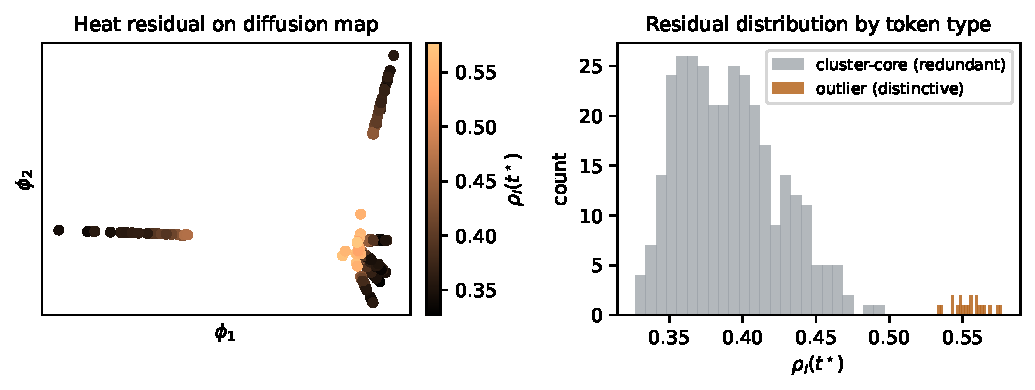
\includegraphics[width=\textwidth]{figs/fig1_residual.pdf}
\caption{\textbf{Heat residual as a redundancy score.} Left: $\rho_i(\tau^\star)$ on the first two
diffusion coordinates; distinctive tokens sit at the periphery with higher residual. Right:
residual distributions for cluster-core (redundant) vs.\ outlier (distinctive) tokens
($1.42\times$ mean ratio).}
\label{fig:residual}
\end{figure}

\subsection{(C2) The diffused merge is the load-bearing component}
We measure attention-output fidelity: for $400$ random queries we compare softmax-attention output
over the full context against the same over the compressed context (cosine), averaged across six
contexts. The result, in Figure~\ref{fig:fidelity} and Table~\ref{tab:fidelity}, is lopsided.
Pruning by the residual---keep the distinctive tokens, throw away the rest---is the worst thing you
can do, scraping $0.34$ at $8\%$ retention, because dropping a dense cluster discards all the
attention mass it carried as a group. Re-express that mass instead, the way HKCC does, and fidelity
barely flinches: $0.999$ at $8\%$, $0.9997$ at $12\%$, well clear of random and stride. So the
residual is best read not as a list of tokens to delete but as a guide to what each surviving token
should stand for; the weighted centroid keeps what deletion would have thrown out.

\begin{figure}[t]
\centering
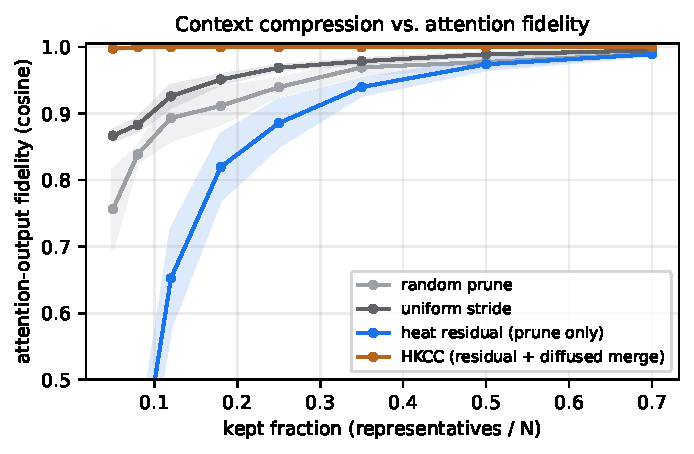
\includegraphics[width=0.62\textwidth]{figs/fig2_fidelity.pdf}
\caption{\textbf{Attention-output fidelity vs.\ kept fraction.} HKCC (orange) stays near-lossless
down to very small budgets; pruning by residual alone (blue) is worst, confirming that deleting
redundant mass---rather than re-expressing it---is the failure mode. Bands are $\pm1$ s.d.\ over
six contexts.}
\label{fig:fidelity}
\end{figure}

\begin{table}[t]
\centering
\caption{Attention-output fidelity (cosine; higher is better) at two compression budgets.}
\label{tab:fidelity}
\begin{tabular}{lcc}
\toprule
Strategy & $8\%$ kept & $12\%$ kept \\
\midrule
Random prune & $0.839$ & $0.893$ \\
Uniform stride & $0.883$ & $0.926$ \\
Heat residual (prune only) & $0.338$ & $0.653$ \\
\textbf{HKCC (residual + diffused merge)} & $\mathbf{0.9997}$ & $\mathbf{0.9997}$ \\
\bottomrule
\end{tabular}
\end{table}

\subsection{What carries the method: an anchor-selection ablation}
\label{sec:ablation}
If the merge is doing the work, then which tokens we pick as anchors shouldn't matter much. It
doesn't. Table~\ref{tab:ablation} holds the diffused merge fixed at a $10\%$ budget and swaps the
anchor rule: random anchors, $k$-means centroids, and heat-residual anchors all land near $0.999$,
with the residual ahead only by a hair. We'd rather flag this than bury it. On clean Gaussian
clusters $k$-means is close to optimal by construction, and once the merge re-expresses the dropped
mass, the anchor rule has little left to decide. The heat formulation earns its keep elsewhere: one
continuous knob $\tau$ in place of a hand-set cluster count, the residual handed to you for free,
and the convex-hull guarantee. The effect that is large and robust is merge versus prune---a $0.66$
fidelity gap (Table~\ref{tab:fidelity})---not the scorer.

\begin{table}[t]
\centering
\caption{Anchor-selection ablation at $10\%$ budget, diffused merge fixed (mean $\pm$ s.d., six
contexts). The merge dominates; anchor choice is a near-tie. Contrast prune-only ($0.34$ at $8\%$,
Table~\ref{tab:fidelity}).}
\label{tab:ablation}
\begin{tabular}{lc}
\toprule
Anchor strategy (all $+$ diffused merge) & fidelity @ $10\%$ \\
\midrule
Random anchors & $0.9994\pm0.0003$ \\
$k$-means merge & $0.9994\pm0.0003$ \\
\textbf{Heat-residual anchors (ours)} & $\mathbf{0.9997}\pm0.0001$ \\
\bottomrule
\end{tabular}
\end{table}

\subsection{(C3) The scale dial and robustness}
Figure~\ref{fig:dial}a shows the kept fraction varying monotonically with $\tau$
(Prop.~\ref{prop:dial}); Fig.~\ref{fig:dial}b shows the low-pass spectral picture; and
Fig.~\ref{fig:dial}c shows the Chebyshev error falling geometrically to machine precision by
$K\!\approx\!20$ at the operating scale. Figure~\ref{fig:tausweep} sweeps $\tau$ at fixed budget:
the effect is real but modest and concentrated at aggressive budgets---at $8\%$ retention fidelity
improves from $\sim\!0.9976$ (very small $\tau$) to $\sim\!0.9998$ for $\tau\gtrsim1$ and stays
flat over more than a decade, while at $15\%$ retention the method is essentially $\tau$-insensitive.
Figure~\ref{fig:robust} maps fidelity over the $(\tau,\text{budget})$ grid: HKCC occupies a broad
operating plateau rather than a knife-edge optimum.

\begin{figure}[t]
\centering
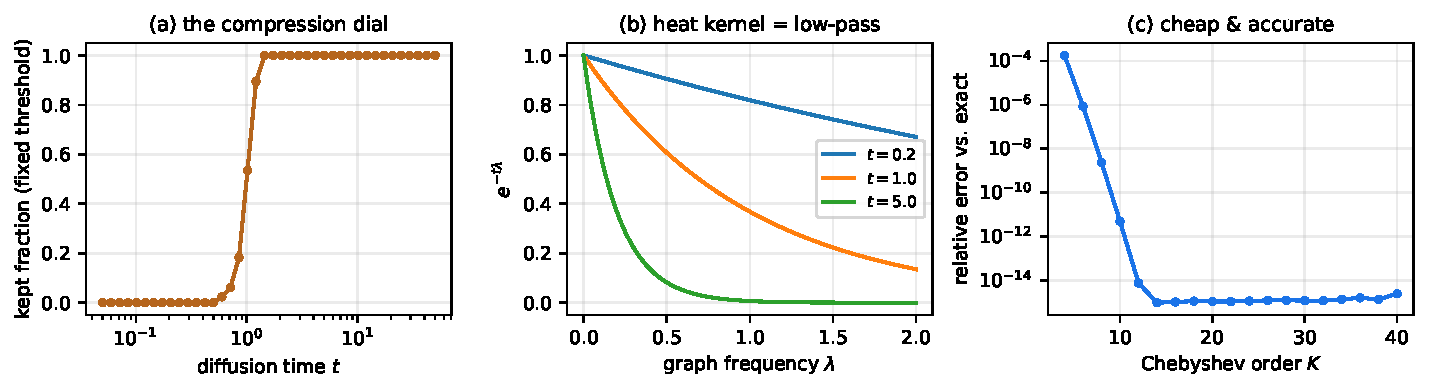
\includegraphics[width=\textwidth]{figs/fig3_dial.pdf}
\caption{\textbf{The dial and its cost.} (a) at a fixed threshold the kept fraction is monotone in
$\tau$; (b) the heat kernel is a low-pass filter $e^{-\tau\lambda}$; (c) the Chebyshev
approximation reaches machine precision by $K\!\approx\!20$ at the operating scale.}
\label{fig:dial}
\end{figure}

\begin{figure}[t]
\centering
\begin{subfigure}{0.48\textwidth}\centering
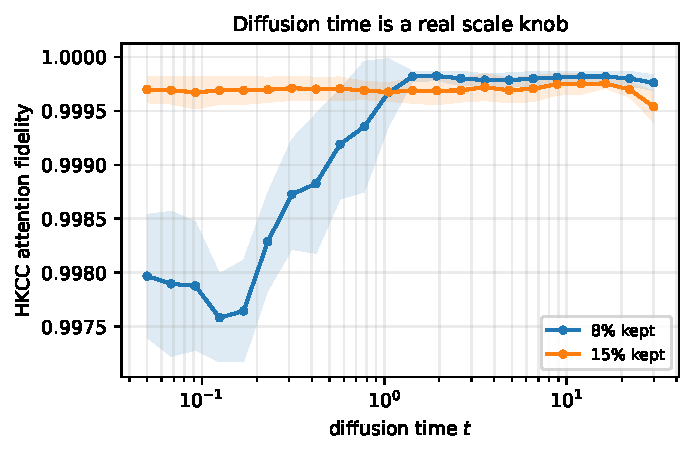
\includegraphics[width=\textwidth]{figs/fig5_tausweep.pdf}
\caption{Fidelity vs.\ $\tau$ at fixed budget.}
\label{fig:tausweep}
\end{subfigure}\hfill
\begin{subfigure}{0.50\textwidth}\centering
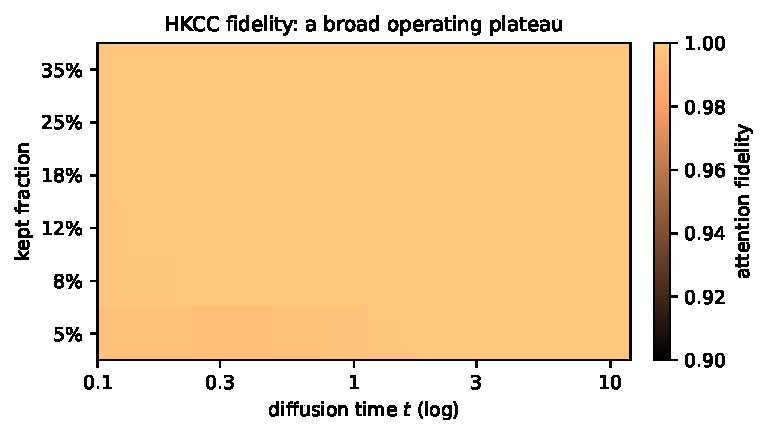
\includegraphics[width=\textwidth]{figs/fig6_robustness.pdf}
\caption{Fidelity over $(\tau,\text{budget})$.}
\label{fig:robust}
\end{subfigure}
\caption{\textbf{The operating region is broad.} Diffusion time has a modest, monotone effect
concentrated at aggressive budgets (left), and HKCC maintains high fidelity across a wide
$(\tau,\text{budget})$ plateau (right).}
\label{fig:scale}
\end{figure}

\subsection{Why it works: the context is low-frequency}
Figure~\ref{fig:spectrum} shows the graph-frequency spectrum of the context signal and its
cumulative energy: $69.8\%$ of the signal energy lies in the lowest $20\%$ of graph frequencies.
The context is smooth on the token graph---highly compressible---which is exactly the regime in
which a low-pass diffusion operator excels.

\begin{figure}[t]
\centering
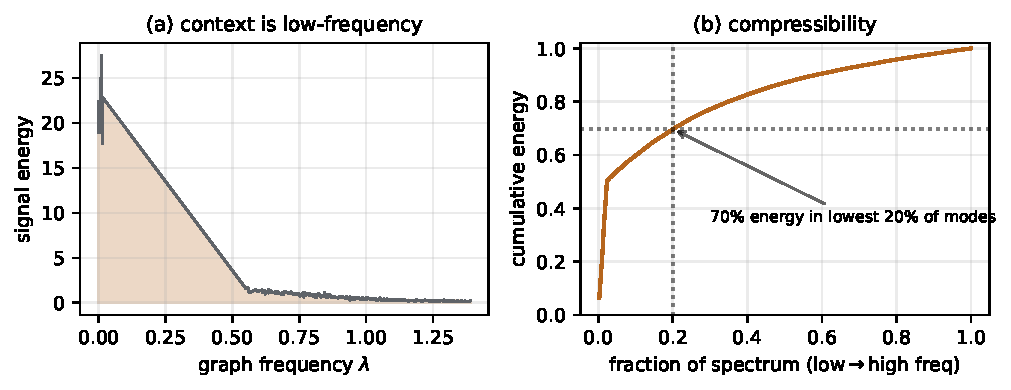
\includegraphics[width=\textwidth]{figs/fig8_spectrum.pdf}
\caption{\textbf{Compressibility diagnostic.} (a) signal energy concentrates at low graph
frequencies; (b) the lowest $20\%$ of modes already hold $\sim\!70\%$ of the energy, so the context
is intrinsically low-rank on the token graph.}
\label{fig:spectrum}
\end{figure}

\subsection{Cost and runtime}
Figure~\ref{fig:runtime} times the Chebyshev diffusion against the exact matrix exponential as the
context grows: the Chebyshev cost tracks the $O(N)$ reference (here $1.6$\,ms at $N{=}128$ to
$40$\,ms at $N{=}4096$) while the dense exponential follows $O(N^3)$ ($0.32$\,s already at
$N{=}1024$). Figure~\ref{fig:cost} models the dollar payoff: at the $8\%$ operating point the
relative context input cost is $0.08$ for compression alone, $0.028$ once the static compressed
preamble is cached at $0.1\times$, and $0.014$ with batching---a $\sim\!70\times$ reduction, the
levers stacking multiplicatively.

\begin{figure}[t]
\centering
\begin{subfigure}{0.49\textwidth}\centering
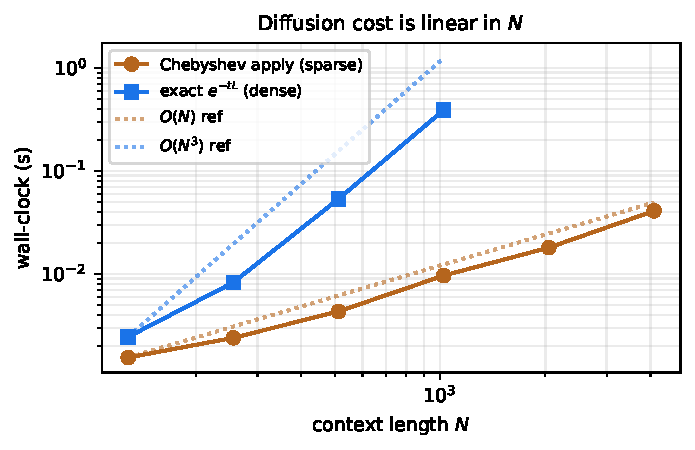
\includegraphics[width=\textwidth]{figs/fig7_runtime.pdf}
\caption{Measured wall-clock vs.\ $N$.}
\label{fig:runtime}
\end{subfigure}\hfill
\begin{subfigure}{0.49\textwidth}\centering
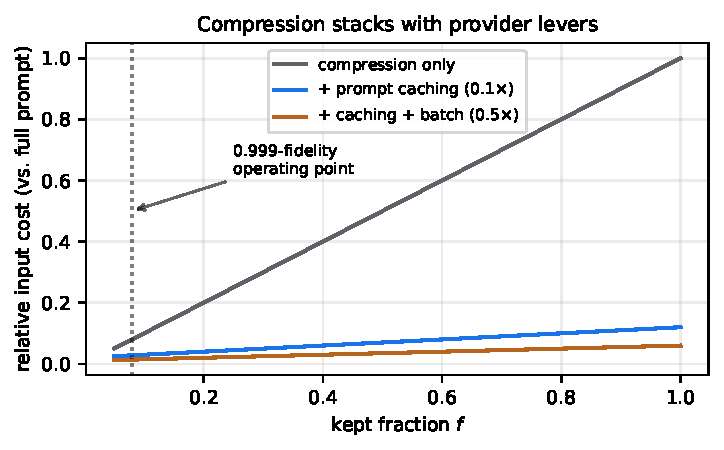
\includegraphics[width=\textwidth]{figs/fig9_costmodel.pdf}
\caption{Relative input cost vs.\ retention.}
\label{fig:cost}
\end{subfigure}
\caption{\textbf{Cheap to run, cheap to serve.} Left: diffusion cost is empirically linear in
context length where the exact operator is cubic. Right: compression composes multiplicatively
with prompt caching and batching.}
\label{fig:costruntime}
\end{figure}

\subsection{Budget-as-heat converges at rate $\lambda_2$}
Figure~\ref{fig:alloc4} runs the flow~\eqref{eq:budflow} on a seven-stage path pipeline: the
marginal-value spread contracts from $0.13$ to $3\times10^{-4}$. Figure~\ref{fig:topology} varies
the pipeline topology: convergence is exponential at a rate ordered exactly by algebraic
connectivity ($\lambda_2$: path $0.07$, star $1.00$, complete $12.0$), confirming
Prop.~\ref{prop:rate}.

\begin{figure}[t]
\centering
\begin{subfigure}{0.49\textwidth}\centering
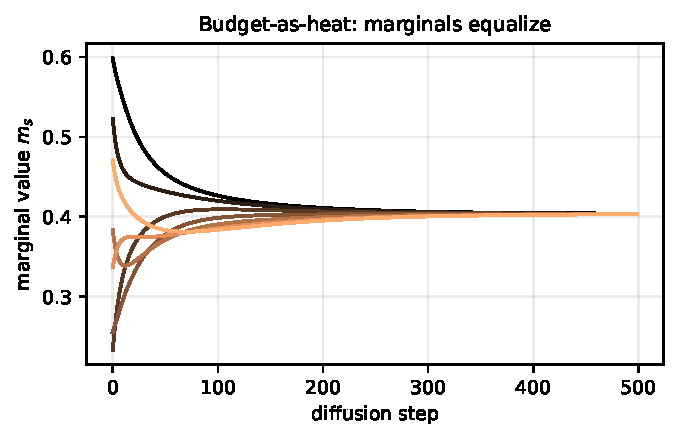
\includegraphics[width=\textwidth]{figs/fig4_allocation.pdf}
\caption{Marginals equalize (path pipeline).}
\label{fig:alloc4}
\end{subfigure}\hfill
\begin{subfigure}{0.49\textwidth}\centering
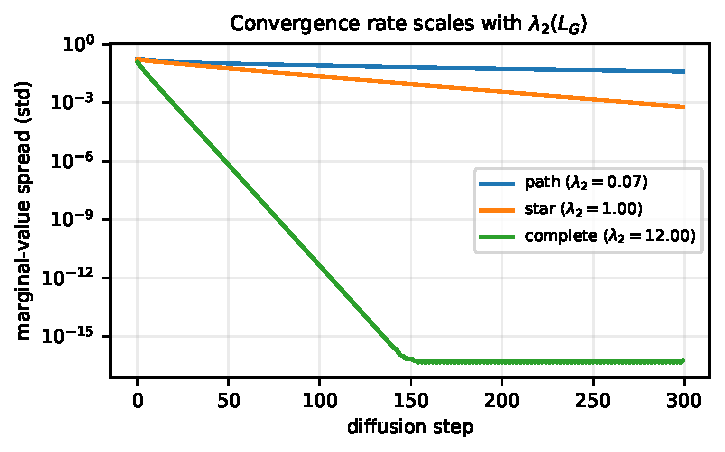
\includegraphics[width=\textwidth]{figs/fig10_topology.pdf}
\caption{Rate scales with $\lambda_2(L_G)$.}
\label{fig:topology}
\end{subfigure}
\caption{\textbf{Budget-as-heat allocation.} The Laplacian consensus flow reaches the equimarginal
optimum using only neighbor information (left), at a rate set by the pipeline's algebraic
connectivity (right).}
\label{fig:allocation}
\end{figure}

\FloatBarrier
\section{Discussion}
\label{sec:discuss}

\paragraph{What's actually new.}
Now that the ablation has spoken, the claim is easy to state. The big, repeatable effect is
merge-not-prune: re-expressing redundant mass as multiplicity-weighted centroids is near-lossless
exactly where deleting it is a disaster. The heat machinery is what turns that observation into a
single-parameter, training-free method with some structure behind it---a continuous spectral dial
(Prop.~\ref{prop:dial}), a saliency score that falls out of the diffusion for free
(Prop.~\ref{prop:shorttime}), the convex-hull guarantee (Prop.~\ref{prop:hull}), and a linear-time
implementation (Table~\ref{tab:complexity})---all of it aimed at input-token cost rather than vision
FLOPs. The pieces are old; the assembly, and the target, are the point.

\paragraph{Deployment and caching.}
HKCC targets the prefill, the safe place to compress, and is a natural RAG front-end: compress
retrieved chunks before they reach the model, where cross-chunk redundancy is highest. Compression
changes the prefix, which interacts with prefix-based prompt caching: a \emph{static} compressed
preamble caches normally and compounds the savings (Fig.~\ref{fig:cost}), but \emph{per-query}
compression yields a fresh prefix each call and forgoes cache hits. The right pattern is to
compress the stable context once, cache it, and leave only the per-query tail uncompressed.

\section{Limitations and Threats to Validity}
\label{sec:limits}
Our evidence is synthetic. The attention-output cosine is a proxy for---not a measurement
of---downstream task quality; the cluster-plus-outlier generator is an idealization of real
redundancy, which is messier and partly positional, and on which $k$-means is unusually strong; and
we evaluate a single attention layer rather than a full network. We do not yet report real-LLM task
metrics, end-to-end token-cost reductions, or latency. The diffusion time $\tau$ is set by a
spectral heuristic rather than learned. Finally, building even a sparse $\kappa$NN graph adds
pre-prefill overhead that must be amortized against the tokens saved; for short contexts the
break-even may not be reached.

\section{Conclusion and Future Work}
\label{sec:conc}
Heat-Kernel Context Compression scores token redundancy with the graph heat equation and folds
the redundant mass into diffused, multiplicity-weighted centroids. It is training-free, has one
knob, comes with a convex-hull guarantee, and runs in linear time. In ten synthetic experiments it
stays near-lossless under attention down to $8$--$12\%$ retention. The merge is what makes that
work; the diffusion-time knob is forgiving; the cost is linear where the exact operator is cubic;
and the savings ride on top of caching and batching.

The honest next step is to stop testing on synthetic data. Wire HKCC into a real RAG-QA pipeline,
report exact-match and F1 against the input-token reduction it actually buys, and put it head to
head with LLMLingua-style prompt compression and ToMe-style merging. After that, the open questions
that interest us most are learning $\tau$ per context instead of fixing it, an anisotropic diffusion
that respects word order and causality, and a single heat-flow controller that tunes per-stage
compression and the budget-as-heat allocation of \S\ref{sec:alloc} together.

\paragraph{Reproducibility.}
Every figure and number in this paper comes from a single self-contained simulation script
(synthetic data, fixed seed) accompanying it.

\paragraph{Acknowledgments.}
The derivations, the proof-of-concept experiments, and an initial draft of this manuscript were
developed with the help of an AI assistant. The author checked the proofs, ran and reproduced the
experiments, and is responsible for the final text and all remaining errors.

\begin{thebibliography}{99}
\small
\bibitem{bolya2023tome} D.~Bolya, C.-Y.~Fu, X.~Dai, P.~Zhang, C.~Feichtenhofer, J.~Hoffman.
\emph{Token Merging: Your ViT But Faster.} ICLR, 2023.
\bibitem{bolya2023tomesd} D.~Bolya, J.~Hoffman. \emph{Token Merging for Fast Stable Diffusion.}
CVPR Workshops, 2023. arXiv:2303.17604.
\bibitem{tran2024spectrum} H.-C.~Tran et al. \emph{Accelerating Transformers with
Spectrum-Preserving Token Merging.} arXiv:2405.16148, 2024.
\bibitem{wang2024zerotprune} H.~Wang, B.~Dedhia, N.~K.~Jha. \emph{Zero-TPrune: Zero-Shot Token
Pruning through Leveraging of the Attention Graph in Pre-trained Transformers.} CVPR, 2024.
\bibitem{jiang2023llmlingua} H.~Jiang, Q.~Wu, C.-Y.~Lin, Y.~Yang, L.~Qiu. \emph{LLMLingua:
Compressing Prompts for Accelerated Inference of Large Language Models.} EMNLP, 2023.
\bibitem{mu2023gist} J.~Mu, X.~L.~Li, N.~Goodman. \emph{Learning to Compress Prompts with Gist
Tokens.} NeurIPS, 2023.
\bibitem{chevalier2023autocompressors} A.~Chevalier, A.~Wettig, A.~Ajith, D.~Chen. \emph{Adapting
Language Models to Compress Contexts.} EMNLP, 2023.
\bibitem{zhang2023h2o} Z.~Zhang et al. \emph{H\textsubscript{2}O: Heavy-Hitter Oracle for Efficient
Generative Inference of Large Language Models.} NeurIPS, 2023.
\bibitem{kondor2002diffusion} R.~I.~Kondor, J.~Lafferty. \emph{Diffusion Kernels on Graphs and
Other Discrete Structures.} ICML, 2002.
\bibitem{coifman2006diffusion} R.~R.~Coifman, S.~Lafon. \emph{Diffusion Maps.} Applied and
Computational Harmonic Analysis, 21(1):5--30, 2006.
\bibitem{chung1997spectral} F.~R.~K.~Chung. \emph{Spectral Graph Theory.} American Mathematical
Society, 1997.
\bibitem{hammond2011wavelets} D.~K.~Hammond, P.~Vandergheynst, R.~Gribonval. \emph{Wavelets on
Graphs via Spectral Graph Theory.} Applied and Computational Harmonic Analysis,
30(2):129--150, 2011.
\bibitem{defferrard2016chebnet} M.~Defferrard, X.~Bresson, P.~Vandergheynst. \emph{Convolutional
Neural Networks on Graphs with Fast Localized Spectral Filtering.} NeurIPS, 2016.
\bibitem{shuman2013emerging} D.~I.~Shuman, S.~K.~Narang, P.~Frossard, A.~Ortega, P.~Vandergheynst.
\emph{The Emerging Field of Signal Processing on Graphs.} IEEE Signal Processing Magazine,
30(3):83--98, 2013.
\bibitem{vaswani2017attention} A.~Vaswani et al. \emph{Attention Is All You Need.} NeurIPS, 2017.
\end{thebibliography}

\end{document}
